\chapter{Ingeniería de Requerimientos}\label{ch:ingenieriaDeRequerimientos}

En este capítulo, detallaremos el proceso que hemos seguido para identificar, desarrollar y validar los requerimientos de nuestra solución. 
En la ingeniería de requerimientos, utilizamos el marco de trabajo de Design Thinking durante los primeros tres meses, correspondientes al Sprint 0, 
para definir los requerimientos y la arquitectura de la solución.
Posteriormente, a medida que avanzaba el proyecto, se realizaron iteraciones en las etapas de prototipado y prueba cuando se necesitaba refinar más 
algún otro requisito, para este fin, se llevó a cabo un trabajo en paralelo, sin necesidad de repetir todo el proceso completo de Design Thinking.
Como resultado del proceso de Design Thinking, se confeccionó el product backlog de este proyecto. Este backlog fue el fruto de un trabajo exhaustivo 
de validación con el cliente, donde se abordaron y priorizaron los elementos clave del alcance del proyecto. Una vez identificadas y refinadas las necesidades 
y requerimientos a través de las etapas del Design Thinking, el equipo pudo definir claramente las funcionalidades que debían ser desarrolladas. Así, el product 
backlog emergió como una lista priorizada y acordada de tareas y funcionalidades, sirviendo como la hoja de ruta que guió el desarrollo del proyecto.


\section{Etapas de \textit{Design Thinking}}\label{sec:etapasDeDesignThinking}

A continuación se mencionan las técnicas de relevamiento utilizadas durante la etapa de discovery, sus objetivos y resultados obtenidos de aplicar cada una de ellas.

\subsection{Empatizar}

El objetivo principal en esta etapa fue comprender profundamente a los usuarios finales del sistema, especialmente a los miembros de la Guardia del MRCC UY. Se puso 
especial énfasis en entender cómo se manejan los incidentes de búsqueda y rescate, y cuáles son los puntos de dolor en los procesos actuales.

\textbf{Hipótesis Inicial del Problema para la Etapa de Empatizar:}\\
"El proceso de cálculo del área probable de búsqueda en el MRCC demora aproximadamente 20 minutos, lo que provoca retrasos significativos en la gestión de incidentes 
de búsqueda y rescate marítimo. Esta demora afecta la capacidad de respuesta rápida del MRCC durante operaciones críticas, comprometiendo la efectividad de las acciones de rescate."


\textbf{Investigación previa}\\
La investigación previa sobre el sistema SAR y los documentos relacionados, como el Manual IAMSAR, el Plan SAR Marítimo Nacional y el Decreto 506/994, permitió obtener un panorama 
completo sobre los marcos legales, operativos y organizativos que rigen las operaciones de búsqueda y rescate en Uruguay. 
Esta revisión destacó la importancia de la coordinación internacional bajo el Convenio SOLAS, la correcta utilización de patrones de búsqueda estandarizados y la planificación eficiente 
de las misiones SAR en cinco etapas clave. Además, se subrayó la necesidad de contar con recursos bien organizados, simulacros anuales para mantener la preparación, y una comunicación efectiva, 
tanto interna como externa, para garantizar el éxito de las operaciones. 
Con este contexto, la planificación de entrevistas puede enfocarse en identificar los puntos críticos de mejora, optimizar procesos y modernizar las herramientas de gestión SAR.

\textbf{Entrevistas}\\
En esta etapa, realizamos entrevistas a usuarios típicos para obtener una aproximación al problema inicial que buscamos solucionar. Al analizar los perfiles de los participantes, identificamos roles 
distintos.
Las entrevistas al Capitán Hugo de Barros y Guillermo Rodríguez, quienes ocupan roles distintos dentro del Maritime Rescue Coordination Center (MRCC), permitieron una comprensión empática y 
multidimensional de los desafíos en la gestión de incidentes de búsqueda y rescate marítimo. 
El objetivo principal de estas entrevistas fue capturar tanto la perspectiva estratégica de un experto como la operativa de un operador con amplia experiencia, asegurando que se abordarán las 
necesidades y dolores específicos de cada nivel dentro del MRCC. 
Al incluir a ambos usuarios, se logró una visión integral que resalta la importancia de soluciones tecnológicas que no solo optimicen la eficiencia y precisión operativa, sino que también 
faciliten la capacitación continua y mejoren la toma de decisiones en tiempo real, respondiendo de manera efectiva a las necesidades reales del personal del MRCC.

\textbf{Customer Journey Map}\\
El propósito de realizar la inmersión en el Maritime Rescue Coordination Center (MRCC) fue obtener una comprensión de las experiencias de los operadores durante la guardia. Al participar y 
observar directamente sus tareas y desafíos cotidianos, buscamos recopilar información detallada para construir un Customer Journey Map que refleja fielmente el proceso y las necesidades de los 
distintos perfiles.\\
Por qué Aplicamos la Técnica:
\begin{itemize}
    \item \textbf{Construir Empatía Auténtica:} Al vivir la experiencia junto a los operadores, pudimos sentir y comprender las presiones, urgencias y responsabilidades que enfrentan, lo que nos permite 
    conectar emocionalmente con sus necesidades y preocupaciones.
    \item \textbf{Identificar Necesidades Latentes:} Muchas veces, los desafíos y obstáculos no son plenamente articulados en entrevistas formales. La observación directa nos permitió identificar 
    problemas subyacentes y oportunidades de mejora que no son evidentes a simple vista.
    \item \textbf{Validar y Profundizar Hallazgos Previos:} Complementar la información obtenida en entrevistas anteriores con observaciones en el entorno real de trabajo, asegurando una comprensión 
    integral y precisa de las situaciones que enfrentan.
    \item \textbf{Contextualizar el Uso de Herramientas y Procesos:} Entender cómo interactúan con los sistemas actuales, cómo manejan la información y cómo se comunican entre ellos, lo que es esencial 
    para diseñar soluciones que se integren eficazmente en su flujo de trabajo.
\end{itemize}

Lo que Esperábamos Obtener:

\begin{itemize}
    \item \textbf{Insights Profundos y Accionables:} Obtener información detallada sobre los puntos de dolor, ineficiencias y desafíos específicos que enfrentan durante la gestión de incidentes, para 
    orientar el diseño de soluciones efectivas.
    \item \textbf{Mejorar la Eficacia de las Soluciones Propuestas:} Asegurar que las recomendaciones y desarrollos futuros estén alineados con las necesidades reales y cotidianas del personal del MRCC, 
    aumentando la probabilidad de adopción y éxito.
    \item \textbf{Fortalecer la Relación con los Usuarios:} Al demostrar un interés genuino por entender su trabajo y desafíos, fomentamos una relación de confianza que facilita la colaboración y 
    receptividad hacia cambios e innovaciones.
    \item \textbf{Desarrollar una Perspectiva Centrada en el Usuario:} La inmersión nos permite mantener al usuario en el centro del proceso de diseño, garantizando que las soluciones no solo sean 
    técnicamente viables sino también relevantes y útiles para quienes las utilizarán.
\end{itemize}



\subsection{Definir}\\
Aclarar y focalizar las necesidades y lograr la comprensión profunda (insights) de lo que hemos detectado durante la etapa de Empatía.  Identificar temas interesantes y patrones recurrentes, comenzar a 
Identificar Perfiles (Personas) para Identificar necesidades e Insights para los temas.

\textbf{Compartir y capturar}\\
Con el objetivo de consolidar y organizar la información obtenida durante la fase de Empatía, realizamos la actividad de “Compartir y Capturar”.
La actividad de "Compartir y Capturar" es esencial para transformar los hallazgos de la fase de empatía en información accionable. Al compartir nuestras observaciones y capturar los aspectos más relevantes 
sobre los usuarios, estamos construyendo una base sólida para definir con precisión el problema que queremos resolver. Esto nos permitirá diseñar soluciones efectivas y centradas en las personas, alineadas 
con las necesidades y desafíos identificados en nuestra investigación.

\textbf{Saturar y agrupar}
Con el objetivo de Identificar temas interesantes y patrones recurrentes, realizamos la actividad de “Saturar y agrupar”. Para visualizar de manera efectiva los problemas y oportunidades identificados, es 
esencial agrupar físicamente los post-its.\\
Este proceso facilita la identificación de temas recurrentes y patrones comunes, lo que a su vez ayuda a enfocar los esfuerzos en las áreas más críticas. La saturación garantiza que se ha capturado toda la 
información relevante, mientras que la agrupación facilita la identificación de temas y patrones esenciales.\\
Este enfoque estructurado no solo mejora la comprensión de los desafíos existentes, sino que también sienta las bases para el desarrollo de soluciones efectivas y colaborativas.


\textbf{Identificar Perfiles}
Comenzar a identificar perfiles es un paso crucial en el proceso de definir el problema porque nos permite entender profundamente quiénes son los usuarios, qué necesidades tienen y cómo interactúan con el 
contexto en el que se desenvuelven.

Esta técnica nos permitió obtener una versión inicial de necesidades e insights, luego el equipo fue re-escribiendo los mismos y se obtuvieron insights refinados teniendo en cuenta el checklist 
[CREATE INSIGHTS STATEMENTS METHOD CHECKLIST] link https://chrome.google.com/webstore/detail/pdf-viewer/oemmndcbldboiebfnladdacbdfmadadm?hl=pt-BR.


\subsection{Idear}\\


\subsection{Prototipar y Probar}\\


\section{Requerimientos funcionales}\label{sec:requerimientosFuncionales}

\subsection{Formato de historias de usuario}
Los requerimientos funcionales fueron especificados a través de las historias de usuario siguiendo el siguiente formato que cumple con el definition of ready:

\begin{itemize}
    \item \textbf{Como:} Esta parte identifica quién es el usuario o rol específico que se beneficiará de la funcionalidad.
    \item \textbf{Quiero:} Aquí se describe la acción, tarea o funcionalidad que el usuario desea realizar. Debe ser una acción concreta y específica que permita 
    al usuario alcanzar un objetivo o resolver un problema.
    \item \textbf{Para:} Esta parte explica la razón o el beneficio que el usuario obtendrá al realizar la acción. Responde a la pregunta de por qué esta funcionalidad es 
    importante para el usuario.
\end{itemize}

A su vez, se utilizó el siguiente formato de escenarios para los criterios de aceptación:

\begin{itemize}
    \item [Nombre de escenario]
    \item \begin{itemize}
        \item Dado [un contexto],
        \item Cuándo [evento],
        \item Entonces [resultado]
    \end{itemize}
\end{itemize}


\subsection{Priorizacion de historias de usuario}

Este proceso se llevó adelante utilizando las reglas de priorización MoSCoW que es una técnica utilizada para categorizar y priorizar los requerimientos o funcionalidades en un proyecto. El acrónimo 
MoSCoW representa cuatro categorías principales:

% generar una lista numerada
\begin{enumerate}
    \item \textbf{Must have (Debe tener):} Estos son los requisitos críticos que son esenciales para el éxito del proyecto. Sin ellos, el proyecto no puede funcionar adecuadamente.
    \item \textbf{Should have (Debería tener):} Son requisitos importantes, pero no esenciales. Aunque su ausencia no detendrá el proyecto, sí afectaría significativamente su valor o eficiencia.
    \item \textbf{Could have (Podría tener):} Son requisitos deseables que, si se implementan, añadirán valor al proyecto, pero que se pueden considerar prescindibles si hay limitaciones de tiempo o recursos.
    \item \textbf{Won't have (No tendrá):} Requisitos que se han identificado pero que no se incluirán en la entrega actual del proyecto. Pueden ser considerados para futuras iteraciones.
\end{enumerate}

Esta clasificación se realizó en la etapa de Conversation, donde se establece un diálogo cercano y colaborativo con el cliente para definir y acordar los detalles de las historias de usuario. 
Durante esta fase, se discuten las necesidades, expectativas y prioridades del cliente, y se clarifican los requisitos de cada historia de usuario.\\
El propósito de esta conversación es asegurarse de que el equipo de desarrollo y el cliente tengan un entendimiento compartido y preciso de lo que se va a construir. Esto incluye aspectos como la 
funcionalidad esperada, los criterios de aceptación, y cualquier limitación o condición especial. Al hacerlo, se busca alinear las expectativas, minimizar malentendidos y asegurar que el producto final 
cumpla con las necesidades reales del cliente. Esta colaboración temprana y continua es clave para el éxito del proyecto, ya que permite adaptar rápidamente las soluciones a los requerimientos del cliente 
a medida que el proyecto avanza.


\subsection{Estimación de historias de usuario}

Para estimar las historias de usuario, se empleó la técnica de Planning Poker, utilizando la secuencia de Fibonacci como referencia para asignar puntos de esfuerzo a cada historia. 
Con el objetivo de obtener una estimación más precisa de la velocidad del equipo, antes de proceder con la estimación de todas las historias de usuario, realizamos un ciclo completo de trabajo. 
Este ciclo permitió medir el tiempo real requerido para completar una historia de usuario, proporcionando así una base más sólida para las estimaciones posteriores. De esta manera, pudimos ajustar mejor 
nuestras estimaciones de esfuerzo y mejorar la precisión en la planificación del proyecto.

\begin{figure}[H]
    \centering
    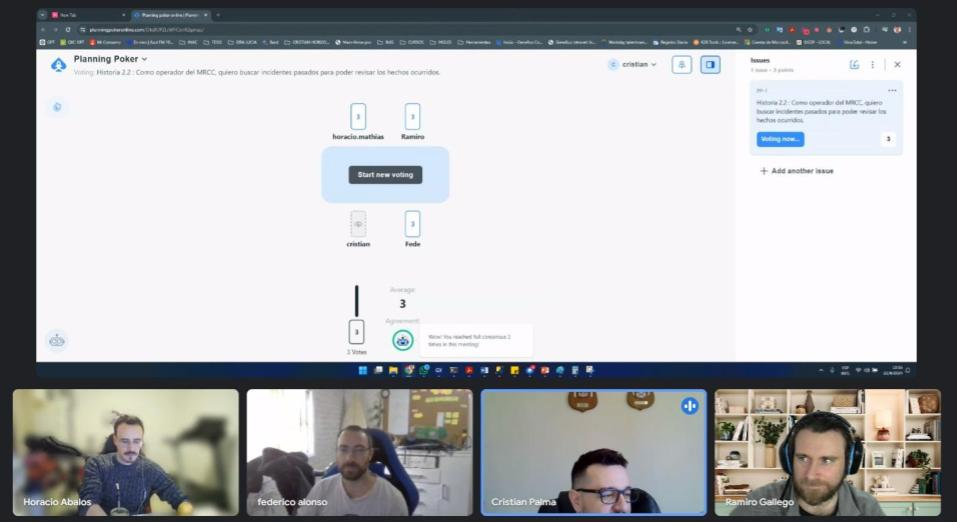
\includegraphics[width=0.8\textwidth]{../imagenes/secciones/4-Ingenieria-de-requerimientos/Poker Planning.jpg}
    \caption{Estimación de historias de usuario con Planning Poker}
    \label{fig:estimacionPokerPlanning}
\end{figure}


\subsection{Product backlog}

A continuación, se muestra un listado que incluye de forma resumida, todas las historias de usuario definidas por el equipo:

\section{Requerimientos no funcionales}\label{sec:requerimientosNoFuncionales}

A partir de los requerimientos no funcionales, se definieron atributos de calidad que a se explicarán en el capítulo de Arquitectura: 

\subsection{Availability}

\textbf{RNF-01}\\
El sistema deberá garantizar alta disponibilidad y resiliencia operativa, pudiendo funcionar 24/7 sin interrupciones (deben poder seguir gestionando el incidente en un ambiente local, 
sin conexión a internet), incluso durante cortes de energía o de red. Debe incluir mecanismos de failover automático y redundancia de datos.


\subsection{Performance}

\textbf{RNF-02}\\
El sistema debe ofrecer tiempos de respuesta rápidos y manejo eficiente de los recursos, especialmente en situaciones críticas y de alta carga operativa.


\subsection{Security}

\textbf{RNF-03}\\
El sistema debe garantizar la privacidad de los datos en flujo. Esto incluye el cifrado de datos en tránsito para prevenir la interceptación y el acceso no autorizado.

\textbf{RNF-04}\\
Los usuarios deberán ser identificados, autenticados y autorizados cada vez que interactúen con la plataforma.

\textbf{RNF-05}\\
El sistema debe mantener la mayor superficie posible de la aplicación de manera privada.

\textbf{RNF-06}\\
Se requerirá uso de roles con distintos privilegios, para controlar el acceso a funcionalidades e información que el sistema maneja. Los roles del sistema son:
\begin{itemize}
    \item Administrador, acceso completo al sistema.
    \item Operador, para gestionar los incidentes.
    \item Jefe, para monitorear los incidentes
\end{itemize}


\subsection{Usability}

\textbf{RNF-07}\\
El sistema debe ser intuitivo y fácil de aprender, permitiendo a los usuarios entender rápidamente si el software es adecuado para sus necesidades.


\subsection{Modifiability}

\textbf{RNF-08}\\
Los cambios de configuración deben poder realizarse sin causar interrupciones significativas en el servicio. Esto incluye la capacidad de actualizar, ajustar y 
mejorar el sistema mientras se mantiene su disponibilidad y funcionalidad operativa.

\textbf{RNF-09}\\
El código y la arquitectura del sistema deben facilitar el mantenimiento y las futuras actualizaciones. Incluir documentación detallada y código fuente comentado 
para apoyar operaciones continuas y desarrollo independiente por parte del equipo de TI de la Armada.


\subsection{Deployability}

\textbf{RNF-10}\\
El sistema debe ser adaptable a diferentes entornos de hardware y software de manera efectiva, asegurando su operación continua y eficiente independientemente de las plataformas subyacentes.

\subsection{Scalability}

\textbf{RNF-11}\\
Capacidad de escalar de manera eficiente para manejar incrementos en la carga de trabajo o en el número de incidentes gestionados simultáneamente sin degradar el rendimiento.

\subsection{Interoperability}

\textbf{RNF-12}\\
El sistema debe poder integrarse con APIs externas para obtener datos meteorológicos y otros datos relevantes en tiempo real.

\section{Restricciones}\label{sec:restricciones}

\textbf{RE01 - Integración en Flujo CI/CD}
El sistema debe estar integrado a un flujo de CI/CD (Integración Continua/Despliegue Continuo) utilizando Jenkins.

\textbf{RE02 - Seguridad del Sistema}
El sistema debe garantizar que, ante un escaneo de seguridad básico, no contiene vulnerabilidades.